\section{Modélisation}

\section{\newspeak}

\begin{frame}{Le projet Penjili}
\centering
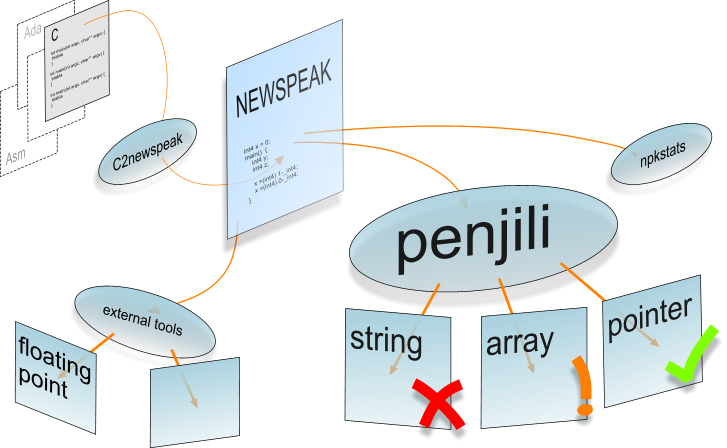
\includegraphics[scale=.5]{img/penjili.png}
\end{frame}

\begin{frame}{Le langage intermédiaire \newspeak}

Un langage adapté à l'analyse statique:

\begin{itemize}
\item simple: il contient peu de constructions
\item explicite: les effets de bords sont explicites
\item expressif: tout programme C peut être converti en \newspeak
\end{itemize}

\end{frame}

\begin{frame}[fragile]{Exemple}

\begin{SaveVerbatim}{compilnpk}
int32 x;
x =(int32) 0;
do {
    while (1) {
        choose {
            -->
                guard((10 > x_int32));
            -->
                guard(! (10 > x_int32));
                goto lbl1;
        }
        x =(int32) coerce[-2**31,2**31-1]
                        (x_int32 + 1);
    }
} with lbl1: {
}
\end{SaveVerbatim}

{\footnotesize
\begin{minipage}{0.3\linewidth}
\insertcode{npk-while.c}
\end{minipage}
\vrule\hspace{2pt}
\begin{minipage}{0.6\linewidth}
\BUseVerbatim{compilnpk}
\end{minipage}
}

\end{frame}

\begin{frame}{Compilation \& analyse}

\begin{tikzpicture}\shorthandoff{!}
\tikzstyle{file}=[draw, shape=rectangle, node distance=2.2cm, minimum
height=1cm, shade, top color=white,
    bottom color=blue!50!black!20, draw=blue!40!black!60, very thick];

\node [file] (c1) {\textcolor{black}{.c}};
\node [file, below of=c1] (c2) {\textcolor{black}{.c}};
\node [node distance=2.2cm, below of=c2] (c3) {};

\node [file, minimum height=0, node distance=5mm, above of=c3,draw] (c3b) {.adb};
\node [file, minimum height=0, node distance=5mm, below of=c3,draw] (c3s) {.ads};

\path (c3b.north west) ++(-3mm,3mm) [draw,dotted] rectangle ($(c3s.south east)+(3mm,-3mm)$);

\node [below of=c3, node distance=2.2cm] (c4){};

\node [file, right of=c1] (cc1) {\textcolor{black}{.c}};
\node [file, right of=c2] (cc2) {\textcolor{black}{.c}};
\node [node distance=2.2cm, right of=c3] (cc3) {};

\node [below of=cc3, node distance=2.2cm](cc4){};

\draw[->] (c1) -- node[above] {{\tiny \ttfamily cpp}} (cc1);
\draw[->] (c2) -- (cc2);

\node [file, right of=cc1] (no1) {\textcolor{black}{.no}};
\node [file, right of=cc2] (no2) {\textcolor{black}{.no}};
\node [file, right of=cc3] (no3) {\textcolor{black}{.no}};

\node [below of=no3, node distance=2.2cm](no4){};

\draw[->] (cc1) -- node[above] {{\tiny \ttfamily c2newspeak -c}} (no1);
\draw[->] (cc2) --  (no2);

\draw[->] ($ (c3b.north east)!0.5!(c3s.south east) + (3mm,0) $) -- node[above] {\tiny \ttfamily ada2newspeak -c} (no3);


\node [file, right of=no2] (npk) {\textcolor{black}{.npk}};

\node [right of=no3, node distance=2.2cm](npk2){};
\node [right of=no4, node distance=2.2cm](npk3){};

\node[draw, ellipse, right of=no2, minimum height=3cm]{};

\draw[->] (no1) -- node {} (npk);
\draw[->] (no2) -- node[above] {{\tiny \ttfamily c2newspeak}} (npk);
\draw[->] (no3) -- node {} (npk);


\node [file, right of=npk, node distance=3cm, yshift=1cm](warn)
    {\textcolor{black}{\parbox{2cm}{\centering Programme \linebreak typé}}};
\node [right of=npk, node distance=3cm, yshift=-1cm](warnn)
    {\textcolor{black}{Erreurs}};

\node [right of=npk3, node distance=3cm](analyser2){};

\node [right of=npk, node distance=3cm] {\small ou};

\draw[->] (npk) -- node[above, yshift=2mm] {{\tiny \ttfamily ptrtype}} (warn);

\draw[->] (npk) -- (warnn);

\draw[->] (c4)   -- node[above, text depth=3pt] {\footnotesize Pr\'etraitement} (cc4);
\draw[->] (cc4)  -- node[above, text depth=3pt] {\footnotesize Compilation} (no4);
\draw[->] (no4)  -- node[above, text depth=3pt] {\footnotesize \'Edition de liens} (npk3);
\draw[->] (npk3) -- node[above, text depth=3pt] {\footnotesize Analyse} (analyser2);
\end{tikzpicture}


% TODO en fait, penjili

\end{frame}


\subsection{\langname}

\begin{frame}{Présentation de \langname}
    \begin{itemize}
        \item C: expressif mais permissif
        \item \newspeak: bon front-end mais bas niveau
        \item \langname = restriction de C \enquote{bien typable}
        \item pas de casts, …
    \end{itemize}
\end{frame}

\begin{frame}{Syntaxe -- Expressions}
  \begin{align*}
  \gramdef{Expressions}{e}
                 { c               }{ Constante }
                 { \opun~e         }{ Opération unaire }
                 { e~\opbin~e      }{ Opération binaire }
                 { lv              }{ Accès mémoire }
                 { lv ← e          }{ Affectation }
                 { \& lv           }{ Pointeur }
                 { \eFun{x_1, …, x_n}{i} }{ Fonction }
                 { e (e_1, …, e_n) }{ Appel de fonction }
                 { \eStruct{
                    l_1 : e_1
                    ; …
                    ; l_n : e_n }  }{ Structure }
                 { \eArray{e_1 ;…; e_n} }{ Tableau }
                 {END}
  \end{align*}
\end{frame}

\begin{frame}{Syntaxe -- Instructions}
  \begin{align*}
  \gramdef{Instructions}{i}
                 { \iPass          }{Instruction vide}
                 { i;i             }{Séquence}
                 { e               }{Expression}
                 { \iDecl{x}{e}{i} }{Déclaration de variable}
                 { \iIf{e}{i}{i}   }{Alternative}
                 { \iWhile{e}{i}   }{Boucle}
                 { \iReturn{e}     }{Retour de fonction}
                 {END}
  \end{align*}
\end{frame}
\subsection{Sémantique}

\begin{frame}{Sémantique impérative}

\begin{itemize}
\item
  Système de transitions entre états
\item
  expression + mémoire
\item
  $\mm{m}{e}{m'}{e'}$
\item expressions $→$ valeurs
\end{itemize}

\end{frame}

\begin{frame}{Valeurs gauches}
    \begin{itemize}
        \item valeurs gauches (\emph{lvalues})
        \item ex: $x.f[2] ← 3$
        \item formes:
            \begin{itemize}
                \item \texttt{x} $→$ \texttt{(n, x)}
                \item \texttt{lv.l} $→ φ.l$
                \item \texttt{lv[e]} $→ φ[n]$
                \item \texttt{*e} $→ φ$
            \end{itemize}
        \item $\mm{m}{lv ← e}{m'}{v}$ ?
    \end{itemize}
\end{frame}

\tikzset{ stackframe/.style={ draw
                            , minimum width=4.5cm
                            }
        }
\tikzset{ twovars/.style={ rectangle split
                         , rectangle split parts=2
                         }
        }

\long\def\figmemstate{
\begin{scope}
    [ start chain=going below
    , every join/.style={<-, thick}
    , node distance=5mm
    ]
    \node[stackframe, on chain, join] (stackbot) {$n ↦ 0$};
    \node[stackframe, on chain, join] {$n ↦ 1$};
    \node[stackframe, on chain, join] {$n ↦ 2$};
    \node[stackframe, on chain, join, twovars]
    (stackf) {\parbox{4.2cm}{ $ x ↦ \left\{
               \begin{array}{ll}
                 f &: \eArray{1;6;1;8}\\
                 g &: 3 \\
               \end{array}
   \right\} $ }
         \nodepart{two} $y ↦ 4$};
    \node[stackframe, on chain, join] (stacktop) {$z ↦ 2$};
\end{scope}
\node[stackframe, twovars, right=5cm of stackbot.north, anchor=north]
    (globvars)
    { $a ↦ 2$ \nodepart{two} $b ↦ 3.14$ };
}

\begin{frame}{Structure de la mémoire}
    \centering
    \begin{tikzpicture}
        \figmemstate{}
    \end{tikzpicture}
\end{frame}

\begin{frame}{Structure de la mémoire}

\begin{itemize}
\item $m = (s, g) ∈ \sMem$
\item $\sMem = \sList{\sFrame} × \sFrame$
\item liste de cadres de pile, cadre de globales
\item cadre: $c = (x_1 ↦ v_1, …, x_n ↦ v_n) ∈ \sFrame$
\item Comment exprimer:
  \begin{itemize}
  \item $m[φ]$
  \item $m[φ←v]$
  \end{itemize}
\end{itemize}
\end{frame}

%\begin{frame}{À la main}
%
%\begin{align*}
%(s, g)[\texttt{Local}~(2, x).f[2] ← 3] &= (s', g) \\
%                   s'_i &= \begin{cases}
%                             s_i & \mbox{ si } i ≠ 2\\
%                             c'  & \mbox{ sinon} \\
%                           \end{cases}\\
%                         c &= s_{2} \mbox{ où } c_i &= (x_i, v_i) \\
%                   c'_i &= (x_i, v'_i) \\
%                   v'_i &= \begin{cases}
%                              v_i &  \mbox{ si } i ≠ 1 \\
%                              3   &  \mbox{ sinon }\\
%                           \end{cases} \\
%                    … & …
%\end{align*}
%\end{frame}

\subsection{Lentilles}

\definecolor{figcola}{HTML}{EFEF52}
\definecolor{figcolb}{HTML}{52EFA1}
\definecolor{figcolc}{HTML}{52A1EF}
\definecolor{figcold}{HTML}{EFA152}

\tikzset{bignode/.style={draw,shape=rectangle,minimum size=1.5cm,fill=figcola}}
\tikzset{smallnode/.style={draw,shape=circle,minimum size=1cm,fill=figcolb}}
\tikzset{trinode/.style={draw,shape=regular polygon,regular polygon sides=3}}

\def\lensNodeBigX#1{
    \vcenter{\hbox{\scalebox{0.5}{
    \begin{tikzpicture}
        \node[bignode, ultra thick] (A) {};
        \node[smallnode, ultra thick, fill=#1] at (A) {};
    \end{tikzpicture}
    } } }
}

\def\lensInnerX#1{
    \vcenter{\hbox{\scalebox{0.5}{
    \begin{tikzpicture}
        \node[smallnode, ultra thick, fill=#1] {};
    \end{tikzpicture}
    } } }
}

\begin{frame}{Lentilles}

\begin{itemize}
\item
  Relation entre objet et sous-objet
\item
  $ℒ ∈ \setLens{R}{A}$
\item
  $ℒ = \begin{cases}           \mathrm{get}_ℒ : R → A \\           \mathrm{put}_ℒ : (A × R) → R \\          \end{cases}$
\item
  $\lensGet{ℒ}{\lensNodeBigX{figcolb}} = \lensInnerX{figcolb}$
\item
  $\lensPut{ℒ}{\lensInnerX{figcold}}{\lensNodeBigX{figcolb}} = \lensNodeBigX{figcold}$
\end{itemize}

\end{frame}

\begin{frame}{Composition de lentilles}

\begin{center}
\begin{tikzpicture}
[node distance=2.5cm
,>=triangle 45
,ultra thick
]
\node[bignode] (A) {};
\node[right of=A,smallnode] (B) {};
\node[right of=B,trinode,fill=figcolc] (C) {};
\node[below of=B,smallnode] (D) {};
\node[below of=A,node distance=5cm,bignode] (E) {};

\draw[->] (A) to node[auto] {$\mathrm{get}_{ℒ_1}$} (B);
\draw[->] (B) to (D);
\draw[->] (A) to (E);
\draw (C) |- node[auto,near end,swap] {$\mathrm{put}_{ℒ_2}$} ($(B)!0.5!(D)$);
\draw (D) |- node[auto,near end,swap] {$\mathrm{put}_{ℒ_1}$} ($(A)!0.75!(E)$);

\node[smallnode] at (A) {};
\node[trinode,fill=figcold] at (A) {};

\node[trinode,fill=figcold] at (B) {};

\node[trinode,fill=figcolc] at (D) {};

\node[smallnode] at (E) {};
\node[trinode,fill=figcolc] at (E) {};

\node[left of=A, node distance=4cm,bignode] (GA) {};
\node[below of=GA,smallnode] (GB) {};
\node[below of=GB,trinode,fill=figcold] (GC) {};

\node[smallnode] at (GA) {};

\node[trinode, fill=figcold] at (GA) {};
\node[trinode, fill=figcold] at (GB) {};

\draw [->] (GA) to node[auto] {$\mathrm{get}_{ℒ_1}$} (GB);
\draw [->] (GB) to node[auto] {$\mathrm{get}_{ℒ_2}$} (GC);

\end{tikzpicture}

\vspace{-1cm}\hspace{7cm} \fbox{$ℒ_1 \ggg ℒ_2$}

\end{center}

\end{frame}

\begin{frame}{Lentilles en sémantique}

    \begin{align*}
       Φ &∈ \sPath → \setLens{Mem}{Val} \\
        \\
       φ &= (2, x).f[2] \\
    Φ(φ) &= \texttt{fst} \ggg I(2) \ggg L(x) \ggg F(f) \ggg T(2) \\
    \end{align*}

\end{frame}

\begin{frame}{Application des lentilles}
    \centering
    \begin{tikzpicture}
        [ highlight/.style={ thick
                           , red
                           }
        ]
        \figmemstate{}

        \path[use as bounding box] ($ (stacktop.south west) + (-3mm, -3mm) $)
                         rectangle ($ (globvars.north east)  + (3mm, 3mm) $);

        \only<2>{
            \draw[highlight] ($ (stackbot.north west) + (-3mm, 3mm) $)
                   rectangle ($ (stacktop.south east) + (3mm, -3mm) $);
        }

        \only<3>{
            \draw[highlight] ($ (stackf.north west) + (-3mm, 3mm) $)
                   rectangle ($ (stackf.south east) + (3mm, -3mm) $);
        }

        \only<4>{
            \draw[highlight] ($ (stackf.north west) + (10mm, 1mm) $)
                   rectangle ($ (stackf.text split east) + (-3mm, -1mm) $);
        }

        \only<5>{
            \draw[highlight] ($ (stackf.north west) + (22mm, -1mm) $)
                   rectangle ($ (stackf.text east) + (-7.5mm, 0) $);
        }

        \only<6>{
            \draw[highlight] ($ (stackf.north west) + (30.3mm, -1mm) $)
                   rectangle ($ (stackf.text east) + (-12.3mm, 0) $);
        }

        \node[below=1cm of globvars] {
            \begin{minipage}{4cm}
            \begin{align*}
                   φ &= \only<2->{(}\only<3->{2,}\only<4->{ x)}\only<5->{.f}\only<6->{[2]} \\
                Φ(φ) &= \only<2->{ \texttt{fst} } \\
         \only<3->{  &\ggg I(2)      \\}
         \only<4->{  &\ggg L(x)      \\}
         \only<5->{  &\ggg F(f)      \\}
         \only<6->{  &\ggg T(2)      \\}
        \hspace{1cm} & \hspace{2.5cm} \\ % align trick...
            \end{align*}
            \end{minipage}
        };
    \end{tikzpicture}
\end{frame}

\begin{frame}{Lentilles en sémantique}
    \centering
    \begin{tabular}{cccl}
        \toprule
        $ℒ$ & R & A & \\
        \midrule
        $I(n)$ & $\sList{α}$     & $α$   & n\ieme élément \\
        $L(k)$ & $\sList{(α×β)}$ & $β$   & liste d'association \\
        $T(n)$ & \sVal           & \sVal & tableau \\
        $F(l)$ & \sVal           & \sVal & structure \\
        $Φ(φ)$ & \sMem           & \sVal & chemin \\
        \bottomrule
    \end{tabular}
\end{frame}

\begin{frame}{Définition de $Φ$}
\begin{align*}
    Φ(v)    &= V(v) \\
  Φ(φ.l)    &= Φ(φ) \ggg F(l) \\
  Φ(φ[n])   &= Φ(φ) \ggg T(n) \\
            & \\
 m[φ]       &\eqdef \lensGet{Φ(φ)}{m} \\
 m[φ ← v]   &\eqdef \lensPut{Φ(φ)}{v}{m} \\
  \end{align*}
\end{frame}

\subsection{Système de types}

% TODO figure statique/dynamique à mettre ici et en intro

\begin{frame}{Système de types}
    \begin{itemize}
        \item Classification statique selon la forme des expressions
        \item $Γ ⊢ e : t$
        \item Monomorphe: un seul type par expression
    \end{itemize}
\end{frame}

\begin{frame}{Système de types}
\begin{align*}
  \gramdef{Type}{t}
      { \tInt                       }{Entier}
      { \tFloat                     }{Flottant}
      { \tUnit                      }{Unité}
      { \ptrK{t}                    }{Pointeur noyau}
      { \ptrU{t}                    }{Pointeur utilisateur}
      { t~[~]                       }{Tableau}
      { \tStruct{ l_1 : t_1; … ; l_n : t_n } }{Structure}
      { (t_1, …, t_n) \rightarrow t }{Fonction}
      {END}
\end{align*}
\end{frame}

\begin{frame}{Deux types de pointeurs}

Pointeurs noyau : $\colK{\ptrK{t}}$

  \begin{itemize}
  \item valeur fixée à la compilation ou par le runtime
  \item ex: \texttt{\&x}, \texttt{malloc(n)}
  \item peuvent être déréférencés (\texttt{*p}, \texttt{memcpy()})
  \end{itemize}

Pointeurs utilisateur : $\colU{\ptrU{t}}$

  \begin{itemize}
  \item valeur provient d'un utilisateur non privilégié
  \item ex: paramètres d'appels systèmes
  \item doivent être vérifiés dynamiquement!
  \end{itemize}

\end{frame}

\begin{frame}{Différence entre les types C et les types inférés}
    \centering
      \begin{tabular}{ll}
          \toprule
          C & \langname \\
          \midrule
          \texttt{int} & $\tInt$ \\
          \texttt{int *} (utilisé \texttt{x[i]}) & $\tInt~[~]$ \\
          \texttt{int *} (utilisé \texttt{*x}) & $\ptrK{\tInt}$ \\
          \texttt{int *} (argument syscall) & $\ptrU{\tInt}$ \\
          \bottomrule
      \end{tabular}
\end{frame}

\begin{frame}{Règles de typage}
    \begin{mathpar}
       \irule{Addr}
         { Γ ⊢ lv : t }
         { Γ ⊢ \& lv : \colK{\ptrK{t}} }

       \irule{Lv-Deref}
         { Γ ⊢ \colK{e} : \colK{\ptrK{t}} }
         { Γ ⊢ \colK{*~e} : t }

       \irule{User-Get}
         { Γ ⊢ \colK{e_d} : \colK{\ptrK{t}}
        \\ Γ ⊢ \colU{e_s} : \colU{\ptrU{t}}
         }
         { Γ ⊢ \uGet{\colK{e_d}}{\colU{e_s}} : \tInt }

       \irule{User-Put}
         { Γ ⊢ \colU{e_d} : \colU{\ptrU{t}}
        \\ Γ ⊢ \colK{e_s} : \colK{\ptrK{t}}
         }
         { Γ ⊢ \uPut{\colU{e_d}}{\colK{e_s}} : \tInt }
    \end{mathpar}
\end{frame}

\begin{frame}{Sûreté du typage}

\begin{theorem}[Progrès]
  Supposons que $Γ ⊢ e : t$. Soit $m$ un état mémoire tel que $\mcomp{Γ}{m}$.
  Alors l'un des cas suivants est vrai:

\begin{itemize}
  \item $∃ v ≠ Ω, e = v$
  \item $∃ (e', m'), \mm{m}{e}{m'}{e'}$
  \item $∃ Ω ∈ \{\serr{div},\serr{array},\serr{ptr}\}, \msi{m}{e} → Ω$
\end{itemize}
\end{theorem}
\end{frame}

\begin{frame}{Sûreté du typage}

\begin{theorem}[Préservation]

Soit $Γ$ un environnement de typage et $m$ un état mémoire tels que
$\mcomp{Γ}{m}$. Soit $e$ une expression telle que $Γ ⊢ e : t$.

Alors, si $\mm{m}{e}{m'}{e'}$, on a $Γ ⊢ e' : t$ et $\mcomp{Γ}{\cCleanup{m'}}$.

\end{theorem}
\end{frame}
